\section{Link Path Loss}\label{sec:reachi-experiments}
In this section, we present the method for simulating link \gls{pathloss} from \cite{paper:linkmodel}, as well
as why the model does not work for our needs. For our own simulations, we want to simulate the performance of
nodes in a \gls{manet}. The performance is, however, heavily dependent on network conditions and the
capabilities of the technology~\cite[p.~10]{paper:linkmodel}. The author of \cite{paper:linkmodel} presents
methods for evaluating the performance of a wireless network, and proceeds to introduce methods for simulating
\gls{pathloss} on a multi-link model, based on real-world performance measurements. \medbreak

The author of \cite{paper:linkmodel} describes the \gls{pathloss} of a link to be the sum of two parts: A
deterministic distance dependent part, that describes the mean signal attenuation at any given link distance,
and a stochastic shadow fading part, which is the \gls{pathloss} caused by terrain, buildings, vegetation and
cars. With this \gls{pathloss} it is possible to simulate the \gls{rssi} on a given link, by subtracting the
\gls{pathloss} from the transmission power of the simulated radio.
%
\begin{eq}\label{eq:ld}
    \mathit{pl}_d(l) = 55 \log_{10}(d(l)) - 18.8
\end{eq}

The distance dependent \gls{pathloss} is computed using the $\mathit{pl}_d(l)$ function shown in
\autoref{eq:ld}~\cite[p.~25]{paper:linkmodel}, where the function $d(l)$ denotes the distance of a link in
meters. Computing the shadow fading \gls{pathloss}, on the other hand, is not as trivial. The shadow fading
part of the \gls{pathloss} is based on the correlation between angles of link pairs sharing a common nodes,
and bears a significant practical limitation in the sense that the shadow fading part depends on a Cholesky
factorisation with a computational complexity of $O(N^6)$~\cite[p.~31]{paper:linkmodel}, where $N$ is the
total number of nodes in the network. \medbreak

Through personal communication with the author of \cite{paper:linkmodel}, we received access to logs from
field experiments for the Reachi project. These field experiments were conducted in different locations with
an early prototype of the Reachi device. The logs contain \gls{gps} coordinates, as well as \gls{rssi}
information for detected neighbours of each node. Examining these logs has shown discrepancies between the
\gls{pathloss} model from \cite{paper:linkmodel} and the measured \gls{rssi}.
\autoref{plot:reachi-experiments:measurements-vs-ld} plots samples drawn from the $\mathit{pl}_d(l)$ function
and measurements from a log containing field measurements from an experiment in Marikina, in the Phillippines.
Since the log contained a total of 17761 links, the measurements are summarised based on the distance of the
link, and each link was sorted into distance buckets with 20 meter intervals. The average \gls{rssi} for all
links in a bucket is plotted in \autoref{plot:reachi-experiments:measurements-vs-ld}. The plot shows that the
\gls{rssi} computed with the distance dependent \gls{pathloss} does not fit with the measured \gls{rssi}.
\medbreak

As mentioned earlier, the shadow fading \gls{pathloss} is based on the correlation between angles of link
pairs that share a common node. An assumption for this is that link pairs with a high correlation, where the
angle between them is low, will have close to the same shadow fading~\cite{paper:linkmodel}. However, this
does not seem to be the case. \autoref{plot:reachi-experiments:avg-rssi-angle-phili-rude} show a plot where we
compare the Marikina log from earlier, with another field experiment log from Rude Skov. For both logs, pairs
of links sharing a common node were sorted, based on the angle between them, into buckets of 5 \degree
intervals, and we computed the average \gls{rssi} for these buckets, after removing the distance dependent
\gls{pathloss}. This means that only the shadow fading part of the \gls{pathloss} is included in the
\gls{rssi} plotted in \autoref{plot:reachi-experiments:avg-rssi-angle-phili-rude}. Under the assumption that a
highly correlated link pairs should result in less shadow fading \gls{pathloss}, the traces on
\autoref{plot:reachi-experiments:avg-rssi-angle-phili-rude} should increase gradually as the angle increases.
This is not the case. \medbreak

Because of this, and the fact that computing the shadow fading path loss is not feasible for a very large
number of nodes, we instead propose our own model for approximating the shadow fading \gls{pathloss}.

%As mentioned above, the angle based approach relies on the assumption that link pairs with a high correlation,
%i.e. low angle between them, will have close to the same shadow fading. We have however not been able to
%produce reliable proof that the assumption is correct. To produce proof, the Marikina and Rude skov log was
%used. 

%For both logs, link pairs were created and sorted based on their angle into separate bucekts of
%5$\degree$ intervals. The average \gls{rssi} for each bucket was then computed. Before computing the average
%\gls{rssi}, the distance dependent part $l_d$ was removed from the links \gls{rssi} measurement, to isolate
%the stochastic part. The resulting data can be seen plotted on
%\autoref{plot:reachi-experiments:avg-rssi-angle-phili-rude}. Under the previous assumption that a high
%correlation gives smaller stochastic path loss, then the traces on
%\autoref{plot:reachi-experiments:avg-rssi-angle-phili-rude} should increase gradually as the angle increases.
%Clearly the measurements does increase as the angle increase, but the increaes are not steady but rather vary
%greatly. Too greatly to say that with certainty that the assumption holds on the received logs.

\begin{figure}[H]
    \centering
    \begin{tikzpicture}
        \begin{axis}[
                height=10.5cm, width=0.95\textwidth,
                ylabel={RSSI},
                xlabel={Distance in meters},
                axis lines*=left,
                xmin=0, xmax=750,
                enlargelimits=false,
                ymin=-120, ymax=-20,
                xtick={0, 50, 100, 150, 200, 250, 300, 350, 400, 450, 500, 550, 600, 650, 700, 750},
                ymajorgrids=true,
                xmajorgrids=true,
                grid style=dashed,
                restrict y to domain=-120:-20,
                samples=600
            ]

            \addplot[very thick, solid, cyan, mark=*] coordinates {(20, -28.32345013477089) (40, -44.85830258302583) (60, -52.77323717948718) (80, -60.21201657458563) (100, -66.47435897435898) (120, -69.68905472636816) (140, -71.5976496922216) (160, -73.7866473149492) (180, -75.53428571428572) (200, -76.89289392378991) (220, -77.88135593220339) (240, -77.8035019455253) (260, -77.36784140969164) (280, -77.14030612244898) (300, -77.75299760191847) (320, -79.71686746987952) (340, -79.15481171548117) (360, -79.90728476821192) (380, -81.30909090909091) (400, -81.79746835443038) (420, -81.52272727272727) (440, -79.2) (460, -79.42105263157895) (480, -79.4375) (500, -79.0) (520, -77.91666666666667) (540, -83.0) (560, -81.27272727272727) (580, -83.57142857142857) (600, -86.0) (620, -83.4) (640, -86.5) (660, -81.42857142857143) (680, -79.0) (700, -82.71428571428571) (740, -77.0)};
            \addlegendentry{Marikina field measurements};

            \addplot[domain=0:740, very thick, solid, red] {26 - ld(x)};
            \addlegendentry{Computed \gls{rssi}};
        \end{axis}
    \end{tikzpicture}
    \caption{Average RSSI pr. distance bucket.}\label{plot:reachi-experiments:measurements-vs-ld}
\end{figure}

\begin{figure}[H]
    \centering
    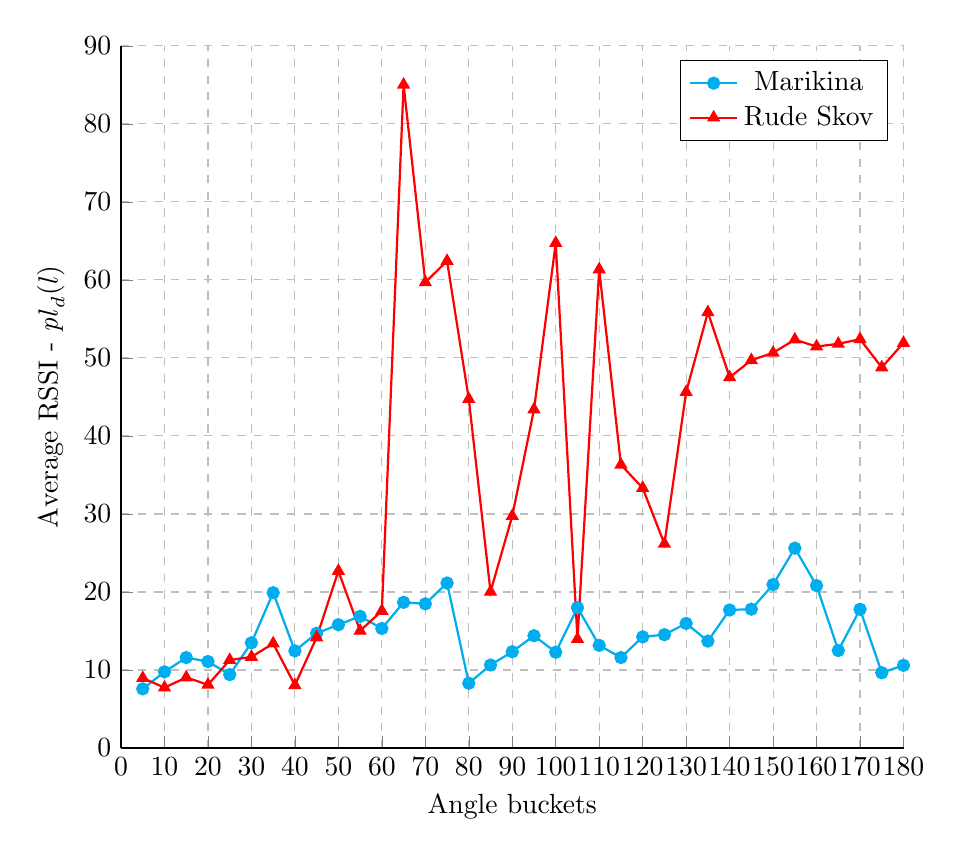
\begin{tikzpicture}
        \begin{axis}[
                height=10.5cm, width=0.95\textwidth,
                ylabel={Average RSSI - $\mathit{pl}_d(l)$},
                xlabel={Angle buckets},
                axis lines*=left,
                xmin=0, xmax=180,
                xtick={0, 10, 20, 30, 40, 50, 60, 70, 80, 90, 100, 110, 120, 130, 140, 150, 160,170,180},
                enlargelimits=false,
                ymin=0, ymax=90,
                ymajorgrids=true,
                xmajorgrids=true,
                grid style=dashed
            ]

            \addplot[thick, solid, cyan, mark=*] coordinates {(5,7.581215097994852)(10,9.763581254686114)(15,11.59234807189617)(20,11.084399582147876)(25,9.411670936293284)(30,13.486232393853125)(35,19.91110051641767)(40,12.453590557884946)(45,14.70313120243339)(50,15.804939314638208)(55,16.87697870999425)(60,15.320902904198922)(65,18.673392004683087)(70,18.48508963612783)(75,21.147550183881993)(80,8.302184073487094)(85,10.641508684206432)(90,12.343183048128944)(95,14.396643466792797)(100,12.27504884861337)(105,17.994872329043496)(110,13.156645245862158)(115,11.595967499573286)(120,14.245146945189493)(125,14.528392002600814)(130,15.96981736460891)(135,13.70427190114752)(140,17.692009757218077)(145,17.79486440192431)(150,20.947579654378668)(155,25.611175147469265)(160,20.819124899373364)(165,12.495568407794714)(170,17.784042978338544)(175,9.646875797269503)(180,10.597197732034614)};
            \addlegendentry{Marikina};


            \addplot[thick, solid, red, mark=triangle*] coordinates {(5,8.968175725354994)(10,7.741408675352775)(15,9.042742837449076)(20,8.108954051047618)(25,11.273321343260399)(30,11.67692967914715)(35,13.401460743255232)(40,8.053793318539391)(45,14.17474549040368)(50,22.68855220716477)(55,15.026896145186285)(60,17.5755161176863)(65,85.01233086400362)(70,59.69038212814202)(75,62.41948703096457)(80,44.72712810089782)(85,20.029080610052482)(90,29.737954905927445)(95,43.39235466255519)(100,64.720015835849)(105,13.965589072181558)(110,61.334883149884675)(115,36.30455538419785)(120,33.32223486902817)(125,26.172354285886417)(130,45.62355888699502)(135,55.8474401182669)(140,47.511612928722954)(145,49.70429537245245)(150,50.649080550831435)(155,52.34402139529124)(160,51.45218633523966)(165,51.805898996936115)(170,52.39131328924595)(175,48.78102582759046)(180,51.91529108595685)};
            \addlegendentry{Rude Skov};
        \end{axis}
    \end{tikzpicture}
    \caption{Average \gls{rssi} per angle bucket without distance dependent \gls{pathloss}.}
    \label{plot:reachi-experiments:avg-rssi-angle-phili-rude}
\end{figure}